% !TeX root = ../main.tex

\section{Electrons in a magnetic field}

\begin{problem}[Onsager formula]
  Suppose that the electron spectrum for a tetragonal lattice can be described
  by the following equation
  \[
    E_k = \frac{\hbar^2 k_x^2}{2m_{xx}} + \frac{\hbar^2 k_y^2}{2m_{xx}}
        + \frac{\hbar^2 k_z^2}{2m_{zz}},
  \]
  with $m_{xx} \neq m_{zz}$. Using the Onsager formula for the cyclotron mass,
  $m_c = \frac{\hbar^2}{2\pi} \pdv A{E_k}$ with $A$ being the area of an
  isoenergetic contour perpendicular to the magnetic field. Find $m_c$ for the
  case when the magnetic field is
  \begin{enumext}[columns = 2]
    \item Along the $z$-axis.
    \item In the $x-y$ plane.
  \end{enumext}
\end{problem}
\begin{solution}\leavevmode
  \begin{enumext}
    \item For $\bm B \parallel \hat z$, the motion of electrons will
    perpendicular to $\hat z$, i.e., parallel to $x-y$ plane. The equation of
    motion becomes
    \[
      E_k = \frac{\hbar^2}{2m_{xx}}(k_x^2 + k_y^2),
    \]
    with the equation of the motion boundary in $k$-space
    \[
      k_\parallel^2 \equiv k_x^2 + k_y^2 = \frac{2m_{xx} E_k}{\hbar^2}.
    \]
    Then, we get the radius. The circle area of the isoenergetic contour is
    \[
      A = \pi k_\parallel^2 = \frac{2\pi m_{xx} E_k}{\hbar^2}.
    \]
    Substituting to the definition of cyclotron mass, we can obtain
    \[
      m_c = \frac{\hbar^2}{2\pi} \pdv A{E_k}
    = \frac{\hbar^2}{2\pi} \frac{2\pi m_{xx}}{\hbar^2} = m_{xx}.
    \]
    \item Simply taking $\bm B \parallel \hat x$, then orbits lie in the
    $k_y-k_z$ plane with an ellipse area. The equation of motion becomes
    \[
      E_k = \frac{\hbar^2 k_y^2}{2m_{xx}} + \frac{\hbar^2 k_z^2}{2m_{zz}},
    \]
    with the equation of the motion boundary in $k$-space
    \[
      \frac{k_y^2}{2m_{xx}E/\hbar^2} + \frac{k_z^2}{2m_{zz}E/\hbar^2} = 1.
    \]
    Then we get the semi-axes. The ellipse area of the isoenergetic contour is
    \[
      A = \pi \sqrt{\frac{2m_{xx}E}{\hbar^2}}
              \sqrt{\frac{2m_{zz}E}{\hbar^2}}
        = \frac{2\pi E}{\hbar^2}\sqrt{m_{xx}m_{zz}}
    \]
    Substituting to the definition of cyclotron mass, we can obtain
    \[
      m_c = \frac{\hbar^2}{2\pi} \pdv A{E_k} = \sqrt{m_{xx}m_{zz}}.
    \]
  \end{enumext}
\end{solution}

\begin{problem}[Integer Quantum Hall Effect]
  The Hall resistance $R_{xy}$ of a two-dimensional electron gas is measured as
  a function of magnetic field $B$ at a very low temperature. A series of
  plateaus are observed at values $R_{xy} = \frac{h}{(\nu e^2)}$, where $\nu$ is
  an integer. Simultaneously, the longitudinal resistance $R_{xx}$ shows peaks
  and drops to zero.
  \begin{enumext}
    \item Explain physically why $R_{xx}$ drops to zero whenever $R_{xy}$ is on
    a plateau.
    \item A sample has an electron density of $n_s = \qty{4.0e11}{\cm^{-2}}$.
    \begin{enumext}
      \item Calculate the filling factor $\nu$ at $B = \qty{2.0}\T$.
      \item What is the expected value of $R_{xy}$ on the plateau nearest to
      this field?
      \item How many Landau levels are completely filled at this plateau?
    \end{enumext}
    \item Why is the IQHE used as a resistance standard? Which two fundamental
    constants are involved?
  \end{enumext}
\end{problem}
\begin{solution}\leavevmode
  \begin{enumext}
    \item When the Hall resistance $R_{xy}$ is on a plateau, the Fermi energy
    lies in a mobility gap between Landau levels. All extended states in the
    bulk are absent, making the bulk insulating. Current flows only along
    dissipationless chiral edge states.
    
    At the edges, backscattering is prevented by spatial separation: even if
    impurities or imperfections exist along an edge, they may cause small
    forward deviations in an electron's path but cannot reverse its direction,
    so no resistance is produced. With no extended states in the bulk to allow
    dissipation and no backscattering at the edges, the longitudinal voltage
    drop vanishes, giving $R_{xx} = 0$.
    \item \begin{enumext}
      \item From the degeneracy of Landau level $n_s = \nu \frac{eB}{h}$,
      we can obtain the filling factor
      \[
        \nu = \frac{n_sh}{eB}
      = \frac{\qty{4.0e15}{\m^{-2}} \times \qty{6.626e-34}{\J\cdot\s}}
          {\qty{1.602e-19}\coulomb \times \qty{2.0}\T} = 8.271.
      \]
      \item Substituting the values into the expression of the Hall resistance
      \[
        R_{xy} = \frac{R_K}{\tilde\nu}
      = \frac{h}{\tilde\nu e^2} = \qty{3226.60}\ohm.
      \]
      where $\tilde \nu$ is the nearest integer of $\nu$.
      \item The filling factor $\tilde \nu = 8$ directly corresponds to the
      number of completely filled Landau levels.
    \end{enumext}
    \item IQHE provides a quantized Hall resistance
    \[
      R_H = \frac{h}{e^2},
    \]
    which precisely quantized and only based on two fundamental constants:
    The Planck constant $h$ and the elementary charge $e$, so it is used as
    a resistance standard.
  \end{enumext}
\end{solution}
\newpage
\begin{problem}[Lifshitz-Kosevich formula]
  The Lifshitz-Kosevich formula describes the amplitude of the Shubnikov-de Haas
  (SdH) oscillations. The amplitude $\Delta R$ is proportional to the factor:
  $R_T = \frac{\lambda(T)}{\sinh \lambda(T)}$,
  where $\lambda(T) = 2\pi^2 \frac{k_BTm^*}{\hbar eB}$.
  \begin{enumext}
    \item A researcher measures the SdH oscillation amplitude $\Delta R$ at a
    fixed magnetic field $B$ as a function of temperature $T$. How can they use
    this data to determine the effective mass $m^*$ of the charge carriers?
    \item Another researcher fixes the temperature $T$ and measures the SdH
    amplitude $\Delta R$ as a function of $1/B$. They find that the amplitude
    decreases exponentially with $1/B$. What physical parameter does this decay
    reveal, and what does a rapid decay imply about the quality of the sample?
  \end{enumext}
\end{problem}
\begin{solution}\leavevmode
  \begin{enumext}
    \item Take $\alpha = \frac{2\pi^2k_Bm^*}{\hbar eB}$,
    then $\lambda(T) = \alpha T$.
    Since at $T \gg 1$, the
    amplitude $\Delta R$ satisfies
    \[
      \Delta R \propto R_T = \frac{\alpha T}{\sinh(\alpha T)}
      \to \frac12 \alpha T \upe^{-\alpha T}, \quad
      \Delta R = \tilde C T\upe^{-\alpha T}
    \]
    Take the logarithm to the two sides
    \[
      \ln \Delta R = \ln \tilde C + \ln T - \alpha T, \quad
      \ln\ab(\frac{\Delta R}T) = -\alpha T + C,
    \]
    where $C = \ln\tilde C$.
    \begin{paracol}{2}
      So, one can take the data at high temperature,
      and use some software tool to convert the original data from
      $T$-$\Delta R$ to $T$-$\ln\ab(\frac{\Delta R}{T})$,
      then plot the new data set like the right figure.
      \switchcolumn \centering
      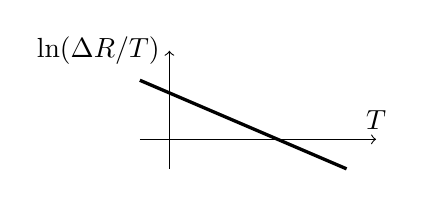
\begin{tikzpicture}[scale = .75]
        \draw [->] (-.5,0) -- (3.5,0) node [above] {$T$};
        \draw [->] (0,-.5) -- (0,1.5) node [left] {$\ln(\Delta R/T)$};
        \draw [very thick] (-.5,1) --++ (3.5,-1.5);
      \end{tikzpicture}
    \end{paracol}
    By fitting the slope $k = -\alpha$ that fits the figure, one can obtain
    the effective mass
    \[
      m^* = \frac{\alpha \hbar eB}{2\pi^2k_B}
    = -\frac{k \hbar eB}{2\pi^2k_B}
    \]
    \item Similarly to part (a), we take $T \gg 1$.
    Since $\Delta R$ is proportional to $R_TR_DR_S$, and if we only
    consider the magnetic variable $B$, then $\Delta R \propto R_TR_D$.
    To be more specific,
    \[
      \Delta R \propto \frac{2\pi^2 k_BTm^*}{\hbar e} \cdot \frac1B \cdot
               \upe^{-\frac{2\pi^2 k_BTm^*}{\hbar e} \cdot \frac1B} \cdot
               \upe^{-\frac{\pi m^*}{e\tau_q} \cdot \frac1B}
    = \tilde C \cdot \frac1B \cdot \upe^{-(\alpha+\beta/\tau_q)\cdot\frac1B}
    \]
    where the coefficients $\alpha$ and $\beta$ can be easily known since we
    have already obtained the effective mass. Taking the logarithm to both
    sides, we can obtain
    \[
      \ln(\Delta R)  = C - \ln B - \ab(\alpha + \frac\beta{\tau_q}) \frac1B,
    \]
    Since the effective mass $m^*$ has been determined from (a), so the
    coefficients $\alpha$ and $\beta$ are known, and the slope directly reveals
    the quantum scattering rate $1/\tau_q$.

    A rapid exponential decay corresponds to a short $\tau_q$, meaning a short
    mean free path and therefore significant disorder: an indicator of poor
    sample quality.
  \end{enumext}
\end{solution}